\documentclass[11pt,a4paper]{article}

% --- Language and fonts
\usepackage[T1]{fontenc}
\usepackage[utf8]{inputenc}
\usepackage[french]{babel}
\usepackage{libertinus}
\usepackage[scaled=0.9]{inconsolata}
\usepackage{microtype}

% --- Page layout
\usepackage[a4paper,margin=2.5cm,headheight=14pt]{geometry}
\usepackage{fancyhdr}
\usepackage{titlesec}
\usepackage{xcolor}
\usepackage{enumitem}
\setlist{itemsep=2pt,topsep=4pt}

% --- Figures and tables
\usepackage{graphicx}
\graphicspath{{figures/}{../assets/}}
\usepackage{booktabs}
\usepackage{longtable}
\usepackage{tabularx}
\usepackage{array}
\usepackage[font=small,labelfont=bf]{caption}
\usepackage{subcaption}
\usepackage[section]{placeins}  % keep floats inside their section
\makeatletter  % stack floats at the top of float-only pages
\setlength{\@fptop}{0pt}
\setlength{\@fpsep}{1.2cm}
\makeatother

% --- Math and code
\usepackage{amsmath}
\usepackage{listings}
\lstset{basicstyle=\ttfamily\small,breaklines=true,columns=fullflexible}

% --- Bibliography and links
\usepackage{csquotes}
\usepackage[backend=biber,style=numeric,sorting=none]{biblatex}
\addbibresource{references.bib}
\usepackage[hidelinks]{hyperref}

% --- Style
\definecolor{cyblue}{HTML}{2A5BA7}
\titleformat{\section}{\Large\bfseries\color{cyblue}}{\thesection}{0.8em}{}
\titleformat{\subsection}{\large\bfseries}{\thesubsection}{0.8em}{}
\titleformat{\subsubsection}{\normalsize\bfseries}{\thesubsubsection}{0.8em}{}

\pagestyle{fancy}
\fancyhf{}
\fancyhead[L]{\small\textcolor{gray}{SignaVision -- Reconnaissance de panneaux de signalisation}}
\fancyhead[R]{\small\textcolor{gray}{CY Tech 2026--2027}}
\fancyfoot[C]{\small\thepage}
\renewcommand{\headrulewidth}{0.4pt}

% Small pictogram used in the class table
\newcommand{\picto}[1]{\raisebox{-0.3\height}{\includegraphics[height=1.3em]{pictograms/#1.png}}}

\newcommand{\auteurs}{Nathan GUIHOT \qquad Elyes DOS SANTOS}

\begin{document}

\begin{titlepage}
  \centering
  
\includegraphics[height=2.2cm]{cytech.png}\par
  \vspace{4cm}
  {\large Fondamentaux du Deep Learning\par}
  \vspace{0.8cm}
  {\color{cyblue}\rule{\linewidth}{0.8pt}}\par
  \vspace{0.4cm}
  {\Huge\bfseries\color{cyblue} SignaVision\par}
  \vspace{0.4cm}
  {\LARGE Reconnaissance automatique\\[0.15cm] de panneaux de signalisation\par}
  \vspace{0.4cm}
  {\color{cyblue}\rule{\linewidth}{0.8pt}}\par
  \vspace{0.6cm}
  {\large Rapport de projet\par}
  \vspace{2.5cm}
  {\large \auteurs\par}
  \vfill
  {Encadrante : Hanane Zerdoum\par}
  \vspace{0.3cm}
  {Octobre 2026\par}
\end{titlepage}

\tableofcontents
\newpage

\section{Introduction}

L'objectif est de reconnaître automatiquement la catégorie d'un panneau de signalisation à partir d'une photo. On traite d'abord la classification d'images contenant un seul panneau déjà recadré, puis, éventuellement, la détection de panneaux dans une scène routière complète. Le code se trouve dans le dossier \texttt{src/} du dépôt.

\section{Données}
\label{sec:donnees}

\subsection{Présentation du jeu de données}

Nous utilisons le \emph{German Traffic Sign Recognition Benchmark} (GTSRB) \cite{stallkamp2011,stallkamp2012}, créé pour une compétition de la conférence IJCNN 2011 et devenu une référence pour la classification de panneaux. Ce sont des photos réelles prises depuis un véhicule, chacune contenant un seul panneau déjà recadré, ce qui correspond au problème des parties 1 à 6 (tableau~\ref{tab:fiche}).

Nous travaillons sur la copie Kaggle \cite{gtsrb_kaggle} : mêmes images que la version officielle \cite{gtsrb_site}, converties en PNG, avec les labels officiels du test (\texttt{GT-final\_test.csv}). Elle a l'avantage de se télécharger directement depuis Colab.

\begin{table}[ht]
  \centering
  \small
  \begin{tabularx}{0.9\linewidth}{@{}lX@{}}
    \toprule
    Auteurs & J. Stallkamp, M. Schlipsing, J. Salmen, C. Igel (INI, Ruhr-Universität Bochum) \\
    Lien officiel & \url{https://benchmark.ini.rub.de/gtsrb_dataset.html} \\
    Version utilisée & \url{https://www.kaggle.com/datasets/meowmeowmeowmeowmeow/gtsrb-german-traffic-sign} \\
    Conditions & Libre d'utilisation, citation demandée (CC0 pour la copie Kaggle) \\
    \midrule
    Images d'entraînement & 39\,209 \\
    Images de test & 12\,630 \\
    Total & 51\,839 \\
    Classes & 43 \\
    Format & PNG, couleur RVB (3 canaux, 8 bits) \\
    Dimensions & Variables, de 25$\times$25 à 266$\times$232 pixels (médiane 43$\times$43) \\
    \bottomrule
  \end{tabularx}
  \caption{Caractéristiques principales du GTSRB.}
  \label{tab:fiche}
\end{table}

Les images d'entraînement sont regroupées en 1\,307 séquences de 30 photos d'un même panneau, prises pendant l'approche du véhicule. Comme ces images sont quasi identiques, la validation devra être séparée par séquence et non image par image, sinon elle serait trop optimiste.

\subsection{Classes}

Le dataset ne fournit que des numéros de classe. La correspondance avec les panneaux (tableau~\ref{tab:classes}) a été établie à partir des pictogrammes de référence fournis, et les classes ont été regroupées en six familles pour l'analyse des résultats.

{\small
\renewcommand{\arraystretch}{1.25}
\begin{longtable}{@{}rcllrr@{}}
  \caption{Les 43 classes du GTSRB et nombre d'images par classe.}
  \label{tab:classes} \\
  \toprule
  N° & & Signification & Famille & Train & Test \\
  \midrule
  \endfirsthead
  \toprule
  N° & & Signification & Famille & Train & Test \\
  \midrule
  \endhead
  \bottomrule
  \endfoot
0 & \picto{0} & Limitation 20 km/h & Limitation de vitesse & 210 & 60 \\
1 & \picto{1} & Limitation 30 km/h & Limitation de vitesse & 2\,220 & 720 \\
2 & \picto{2} & Limitation 50 km/h & Limitation de vitesse & 2\,250 & 750 \\
3 & \picto{3} & Limitation 60 km/h & Limitation de vitesse & 1\,410 & 450 \\
4 & \picto{4} & Limitation 70 km/h & Limitation de vitesse & 1\,980 & 660 \\
5 & \picto{5} & Limitation 80 km/h & Limitation de vitesse & 1\,860 & 630 \\
6 & \picto{6} & Fin de limitation 80 km/h & Fin d'interdiction & 420 & 150 \\
7 & \picto{7} & Limitation 100 km/h & Limitation de vitesse & 1\,440 & 450 \\
8 & \picto{8} & Limitation 120 km/h & Limitation de vitesse & 1\,410 & 450 \\
9 & \picto{9} & Interdiction de dépasser & Interdiction & 1\,470 & 480 \\
10 & \picto{10} & Interdiction de dépasser ($>$ 3,5 t) & Interdiction & 2\,010 & 660 \\
11 & \picto{11} & Priorité à la prochaine intersection & Priorité & 1\,320 & 420 \\
12 & \picto{12} & Route prioritaire & Priorité & 2\,100 & 690 \\
13 & \picto{13} & Cédez le passage & Priorité & 2\,160 & 720 \\
14 & \picto{14} & Stop & Priorité & 780 & 270 \\
15 & \picto{15} & Circulation interdite & Interdiction & 630 & 210 \\
16 & \picto{16} & Accès interdit ($>$ 3,5 t) & Interdiction & 420 & 150 \\
17 & \picto{17} & Sens interdit & Interdiction & 1\,110 & 360 \\
18 & \picto{18} & Danger & Danger & 1\,200 & 390 \\
19 & \picto{19} & Virage à gauche & Danger & 210 & 60 \\
20 & \picto{20} & Virage à droite & Danger & 360 & 90 \\
21 & \picto{21} & Succession de virages & Danger & 330 & 90 \\
22 & \picto{22} & Chaussée déformée & Danger & 390 & 120 \\
23 & \picto{23} & Chaussée glissante & Danger & 510 & 150 \\
24 & \picto{24} & Chaussée rétrécie par la droite & Danger & 270 & 90 \\
25 & \picto{25} & Travaux & Danger & 1\,500 & 480 \\
26 & \picto{26} & Feux tricolores & Danger & 600 & 180 \\
27 & \picto{27} & Passage piétons & Danger & 240 & 60 \\
28 & \picto{28} & Enfants & Danger & 540 & 150 \\
29 & \picto{29} & Cyclistes & Danger & 270 & 90 \\
30 & \picto{30} & Neige ou verglas & Danger & 450 & 150 \\
31 & \picto{31} & Animaux sauvages & Danger & 780 & 270 \\
32 & \picto{32} & Fin de toutes les interdictions & Fin d'interdiction & 240 & 60 \\
33 & \picto{33} & Tourner à droite & Obligation & 689 & 210 \\
34 & \picto{34} & Tourner à gauche & Obligation & 420 & 120 \\
35 & \picto{35} & Tout droit & Obligation & 1\,200 & 390 \\
36 & \picto{36} & Tout droit ou à droite & Obligation & 390 & 120 \\
37 & \picto{37} & Tout droit ou à gauche & Obligation & 210 & 60 \\
38 & \picto{38} & Contournement par la droite & Obligation & 2\,070 & 690 \\
39 & \picto{39} & Contournement par la gauche & Obligation & 300 & 90 \\
40 & \picto{40} & Carrefour giratoire & Obligation & 360 & 90 \\
41 & \picto{41} & Fin d'interdiction de dépasser & Fin d'interdiction & 240 & 60 \\
42 & \picto{42} & Fin d'interdiction de dépasser ($>$ 3,5 t) & Fin d'interdiction & 240 & 90 \\
  \midrule
  \multicolumn{4}{@{}l}{Total} & 39\,209 & 12\,630 \\
\end{longtable}
}
Les photos sont bien plus difficiles à lire que les pictogrammes (figure~\ref{fig:exemples}) : images sombres (classes 8, 20, 41, 42), floues (31), surexposées (40) ou de très faible résolution. Au sein d'une même classe, l'éclairage, l'angle et la netteté varient fortement (figure~\ref{fig:stop}).

\begin{figure}[ht]
  \centering
  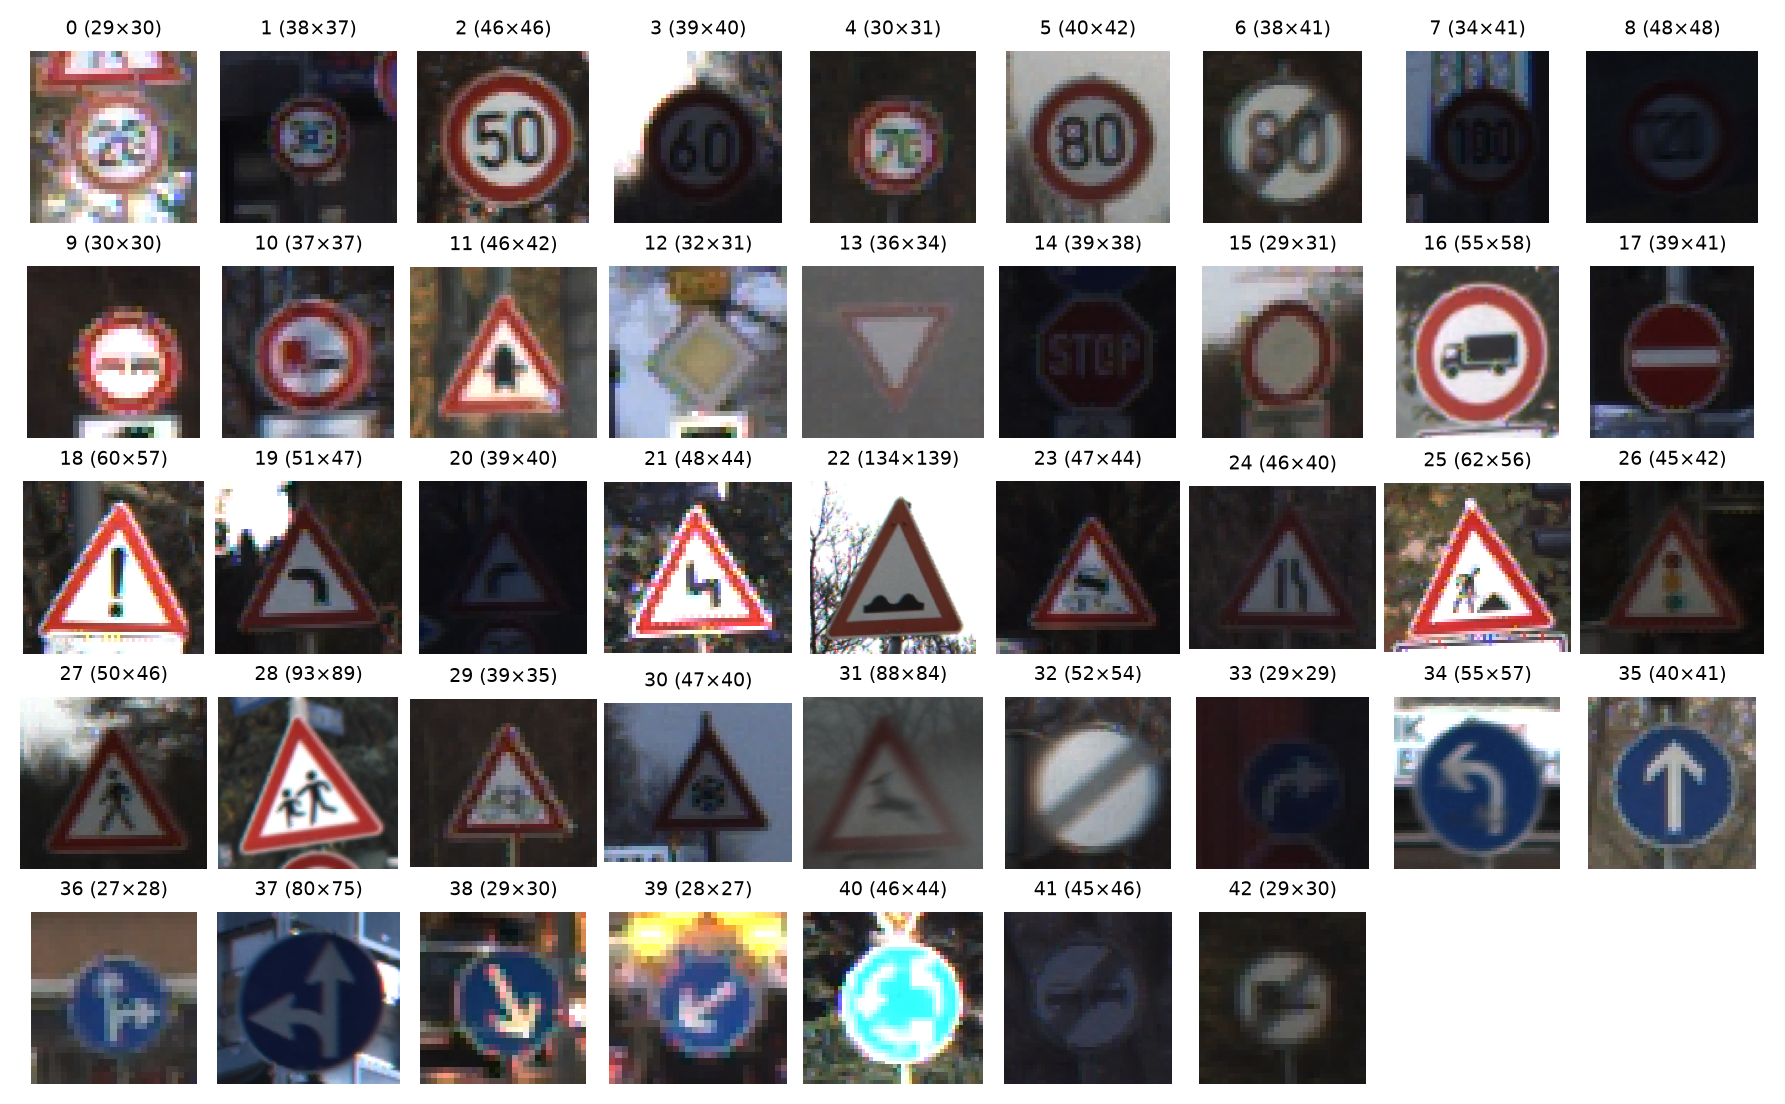
\includegraphics[width=\linewidth]{class_examples.png}
  \caption{Une image d'entraînement tirée au hasard pour chaque classe (numéro de classe et dimensions en pixels).}
  \label{fig:exemples}
\end{figure}

\begin{figure}[ht]
  \centering
  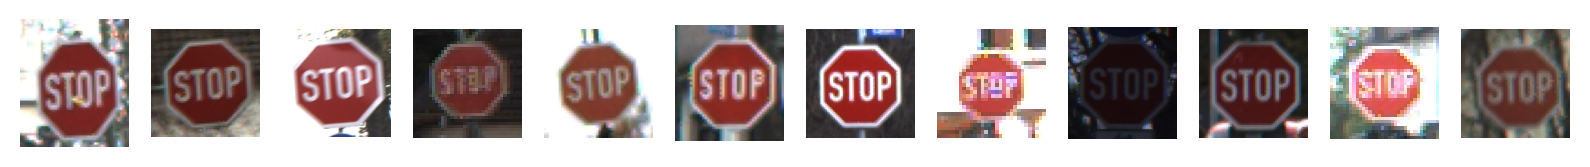
\includegraphics[width=\linewidth]{stop_variability.png}
  \caption{Douze images de la classe 14 (Stop) issues de séquences différentes.}
  \label{fig:stop}
\end{figure}

\subsection{Format et dimensions}

Les images sont presque carrées (rapport largeur / hauteur entre 0,87 et 1,15 pour 95\,\% d'entre elles) et le panneau est entouré d'une marge d'environ 10\,\% \cite{gtsrb_site}. La plupart sont petites (figure~\ref{fig:tailles}) : le plus grand côté ne dépasse pas 59 pixels pour 75\,\% des images, et seules 16,6\,\% ont un côté inférieur à 32 pixels. Le réseau attendant une entrée de taille fixe, toutes les images seront redimensionnées ; 32$\times$32 pixels semble suffisant.

\begin{figure}[ht]
  \centering
  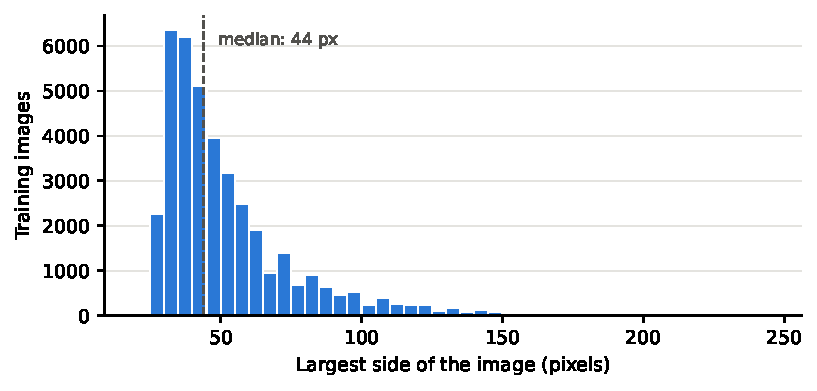
\includegraphics[width=0.6\linewidth]{image_sizes.pdf}
  \caption{Distribution du plus grand côté des images d'entraînement.}
  \label{fig:tailles}
\end{figure}

\subsection{Déséquilibre entre les classes}

Le nombre d'images par classe va de 210 (classes 0, 19 et 37) à 2\,250 (classe 2), soit un rapport de 10,7 (figure~\ref{fig:distribution}). Les limitations de vitesse représentent à elles seules un tiers des images (tableau~\ref{tab:familles}), et le test suit la même répartition. L'accuracy globale sera donc complétée par une matrice de confusion et des résultats par classe ; une pondération des classes pourra être testée lors des expérimentations.

\begin{figure}[ht]
  \centering
  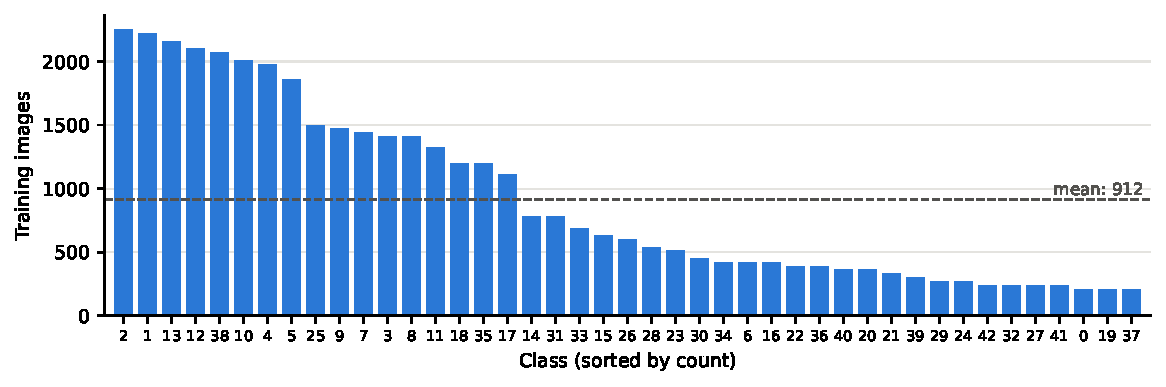
\includegraphics[width=\linewidth]{class_distribution.pdf}
  \caption{Nombre d'images d'entraînement par classe, trié par effectif décroissant.}
  \label{fig:distribution}
\end{figure}

\begin{table}[ht]
  \centering
  \small
  \begin{tabular}{@{}lrrrr@{}}
    \toprule
    Famille & Classes & Train & Test & Part du train \\
    \midrule
    Limitation de vitesse & 8 & 12\,780 & 4\,170 & 32,6\,\% \\
    Danger & 14 & 7\,650 & 2\,370 & 19,5\,\% \\
    Priorité & 4 & 6\,360 & 2\,100 & 16,2\,\% \\
    Interdiction & 5 & 5\,640 & 1\,860 & 14,4\,\% \\
    Obligation & 8 & 5\,639 & 1\,770 & 14,4\,\% \\
    Fin d'interdiction & 4 & 1\,140 & 360 & 2,9\,\% \\
    \bottomrule
  \end{tabular}
  \caption{Répartition des images par famille de panneaux.}
  \label{tab:familles}
\end{table}

% --- TODO: data preparation
% \subsection{Préparation des données}
% - resizing (chosen size + justification)
% - pixel normalization (divide by 255?)
% - label encoding (integers + sparse_categorical_crossentropy, or one-hot)
% - train / validation split by track, test set kept for final evaluation only
% Explain the role of each step.

% \section{Modèle de référence}
\label{sec:baseline}

% Part 2. Dense network: Image -> Flatten -> Dense + activation -> Dense -> Softmax
% To explain:
% - how a color image becomes the input vector
% - weights and biases, forward pass, activation functions
% - loss function, backpropagation, gradient descent
% - softmax output for multi-class classification
% Results: used as a baseline for the CNN.

% \section{Réseau convolutif}
\label{sec:cnn}

% Part 3. Propose and justify the architecture.
% To explain: filters, convolution on 3 channels, feature maps, kernel size,
% stride, padding, ReLU, pooling, Flatten, Dense layers, output layer.
% Layer-by-layer table: output shape + number of parameters.

% \section{Entraînement}
\label{sec:training}

% Part 4. Justify: loss function, optimizer, batch size, number of epochs, metrics.
% Loss / accuracy curves (train and validation) + interpretation, possible overfitting.

% \section{Évaluation et analyse des erreurs}
\label{sec:evaluation}

% Part 5. Evaluation on the test set (once, final model only).
% - confusion matrix, per-class / per-family results
% - well recognized classes, frequent confusions (speed limits?), hardest classes
% - link with brightness, viewing angle, size, blur, similarity between classes
% - examples: image + true class + predicted class + probability, including errors

% \section{Expérimentations}
\label{sec:experiments}

% Part 6. At least 3 experiments, changing a limited number of parameters each time.
% Comparison table: change, validation results, observations.
% Data augmentation: no horizontal flip (it changes the meaning of some signs).
% Justify the choice of the final model.

% \section{Conclusion}
\label{sec:conclusion}

% Summary, limitations, next steps (transfer learning, YOLO detection, video).


\printbibliography[heading=bibintoc,title={Références}]

\end{document}
